\documentclass[titlepage,12pt]{article}

\usepackage[utf8]{inputenc}
\usepackage[a4paper, total={6in, 8in},headheight=14pt]{geometry}
\usepackage{newtxtext,newtxmath}
\usepackage[scaled=1]{couriers}
\usepackage[spanish]{babel}
\usepackage{microtype}
\usepackage[bottom]{footmisc}
\usepackage{fancyhdr}
\usepackage{graphicx}
\usepackage{blindtext}
\usepackage{scrextend}
\usepackage{tocloft}
\usepackage{parskip}
\usepackage{multicol}
\usepackage{subcaption}
\usepackage{wrapfig}
\usepackage{multicol}
\usepackage{verbatimbox}
\usepackage[nottoc, notlot, notlof]{tocbibind}
\usepackage{listingsutf8}
\usepackage{url}
\usepackage[square,numbers]{natbib}
\usepackage{adjustbox}
\usepackage[makeroom]{cancel}
\usepackage[hidelinks]{hyperref}
\usepackage[Glenn]{fncychap}
\usepackage{lastpage}
\usepackage{fancyhdr}

\bibliographystyle{unsrtnat}

\pagestyle{fancy}
\fancyhf{}
\fancyhead[R]{\rightmark}
\fancyfoot[C]{\leftmark}
\fancyfoot[R]{\thepage}
\renewcommand{\footrulewidth}{0.6pt}% Line at the footer visible
\addto\captionscatalan{%
  \renewcommand\contentsname{Índice}%
}

\fancypagestyle{plain}{%
  \fancyhf{}%
  \fancyfoot[R]{\thepage}%
  \renewcommand{\headrulewidth}{0pt}% Line at the header invisible
  \renewcommand{\footrulewidth}{0.6pt}% Line at the footer visible
}


\renewcommand{\cftpartleader}{\cftdotfill{\cftdotsep}}%
\renewcommand{\cftsecleader}{\cftdotfill{\cftdotsep}}%
\renewcommand\familydefault{\sfdefault}

\usepackage{tikz}
\usetikzlibrary{shapes.geometric, arrows}

\newcommand{\Lagr}{\mathcal{L}}
\newcommand{\Xagr}{\mathcal{X}}

\setlength{\skip\footins}{1cm}

\makeatletter
% \patchcmd{<cmd>}{<search>}{<replace>}{<success>}{<failure>}
\patchcmd{\@makechapterhead}{\huge}{\large}{}{}% for \chapter
\patchcmd{\@makechapterhead}{\Huge}{\large}{}{}% for \chapter
\patchcmd{\@makeschapterhead}{\Huge}{\large}{}{}% for \chapter*
\makeatother


\begin{document}

\iftrue
\newcommand{\HRule}{\rule{\linewidth}{0.5mm}}

\thispagestyle{empty}

\begin{center}

{\large Universitat Politècnica de Catalunya}

\medskip
{\large Facultat d'Informàtica de Barcelona (FIB)}

\vfill
{\bfseries\Large Bachelor's Degree Project}

\vfill
\centerline{\mbox{
\includegraphics[width=60mm]{media/FIB_UPC.png}}}

\vfill
\vspace{5mm}

{\LARGE Jordi Gil González}

\vspace{15mm}

% Title in English according to the official assignment
{\LARGE\bfseries Analysis of the Path Tracing \\ rendering method on CPU and GPU}

\normalfont \small \sffamily{}

\vfill

Computer Science Department


\vfill

\begin{tabular}{rl}
Bachelor's Degree Project Director: & Chica Calaf, Antoni \\
\noalign{\vspace{2mm}}
Study programme: & Computer Science\\
\noalign{\vspace{2mm}}
Specialization: & Computer Graphics\\
\end{tabular}

\vfill

\large Academic Year 2019/2020

\large \today

\end{center}

\newpage
\tableofcontents*
\fi

\newpage

\section{Introducción} \label{introduction}

En la actualidad, las imágenes generadas por ordenador están muy presentes tanto en el entorno profesional como en el lúdico. La creación de imágenes realistas mediante el uso de computadoras se ha convertido en una necesidad a la orden del día. Industrias como el cine o los videojuegos requieren de algoritmos capaces de reproducir el mundo real en un entorno virtual y, si siempre que se pueda, en el menor tiempo posible.

El estudio de métodos que permiten renderizar imágenes realistas no es nuevo. Entre principios y mediados de los años 70 comenzaron a publicarse los primeros artículos científicos en referencia a la simulación de la luz y el color sobre superficies modelos tridimensionales. Para poder entender como funcionan estos métodos debemos tener presente la representación de modelos 3D. 

Para representar un modelo 3D se utiliza una ''malla de polígonos'', popularmente conocida como \textit{Mesh} y generalmente estos polígonos suelen ser triángulos. Ésta consiste en un conjunto de vértices conectados por aristas formando caras. Para cada una de estas caras podemos definir un vector normal ortogonal a ésta. En la Figura \ref{dolphin} podemos apreciar un ejemplo de modelo 3D representado por una malla de triángulos.

\begin{figure}[H]
	\centering
	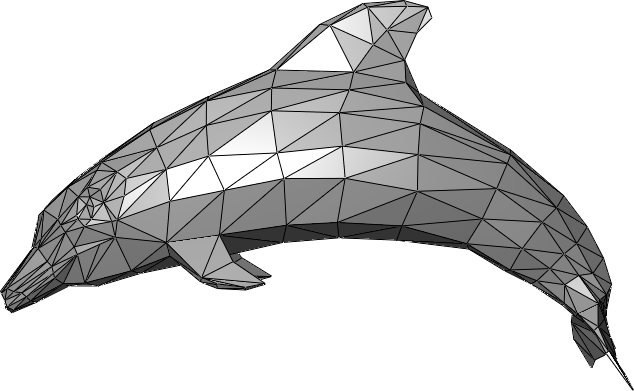
\includegraphics[scale=0.15]{media/Dolphin_triangle_mesh.png}
	\caption{Ejemplo de malla de triángulos. Fuente: Wikipedia}
	\label{dolphin}
\end{figure}

Volviendo a los métodos de cálculo de iluminación, el más simple de todos es el conocido como \textit{Flat Shading}. Para calcular el color de cada una de las caras de nuestra malla solamente tiene en cuenta un vértice de los que la conforman y la normal de ésta, aunque una malla compuesta por triángulos es común utilizar el centroide. El color se interpola para todos los vértices de la cara utilizando el color calculado al inicio dando así un resultado uniforme para toda la cara. Debido a no tener en cuenta las caras adyacentes esto produce resultados diferentes entre ellas. En la Figura \ref{flat:shading} podemos observar el efecto generado por este método. Podríamos pensar que añadir más vértices a nuestra malla los resultados mejorarían, pero no es una propuesta adecuada debido al mayor uso de memoria requerido y el problema no quedaría resuelto. Si hiciéramos \textit{zoom in} en el modelo, volveríamos a apreciar el efecto conocido como ''bandas de Mach'' \citep{Lotto1999}.

\begin{figure}[ht]
	\centering
	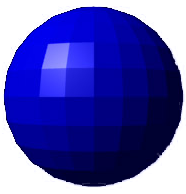
\includegraphics[scale=0.5]{media/Flat-shading-sample.png}
	\caption{Ejemplo de \textit{Flat Shading}. Fuente: Wikipedia}
	\label{flat:shading}
\end{figure}

En los métodos de sombreado suave (\textit{Smooth Shading}), el color cambia de pixel a pixel y no de cara a cara, resultando así en transiciones suaves entre las diferentes caras adyacentes.
En 1971 Henri Gouraud nos presenta en su artículo \textit{Continuous Shading of Curved Surfaces} \citep{Henri1971} el sombreado de Gouraud (\textit{Gouraud Shading}). Este método nos permite añadir mayor continuidad al sombreado respecto al método de \textit{Flat Shading}. El gran avance respecto al método presentado anteriormente es que no precisa de una malla de gran densidad para lograr simular una mayor continuidad. Para cada pixel se determina su intensidad por interpolación de las intensidades definidas en los vértices de cada polígono.

\begin{itemize}
	\item Para cada vértice se define una normal como promedio de las normales de los polígonos a los que pertenece dicho vértice.
	\item Mediante el uso de algún modelo de iluminación como, por ejemplo, el modelo de reflexión de Phong, se calcula la intensidad de cada vértice utilizando la normal obtenida en el punto anterior.
	\item Para cada pixel, se interpola la intensidad en los vértices para obtener la intensidad de éste.
\end{itemize} 

Como podemos observar en la Figura \ref{Gouraud:shading}, los resultados obtenidos respecto el método anterior son notablemente superiores, pero no acaba de representar de forma correcta los reflejos especulares. Éstos puede suponer un problema grave si se presentan en el centro de un polígono (cara) de gran tamaño.

\begin{figure}[ht]
	\centering
	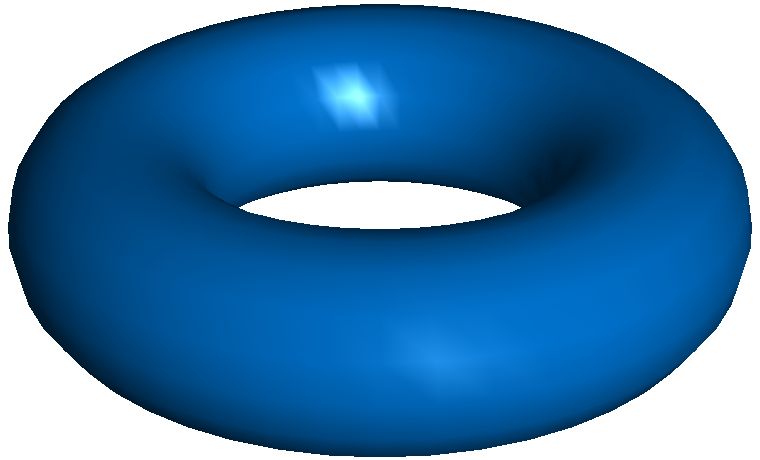
\includegraphics[scale=0.25]{media/Gouraudshading00.png}
	\caption{Ejemplo de \textit{Gouraud Shading}. Fuente: Wikipedia}
	\label{Gouraud:shading}
\end{figure}

Más tarde, Bui Tuong Phong en su tesis doctoral \citep{Phong1975} nos presentaba el sombreado de Phong. En el método presentado por Phong en vez de calcular la intensidad en el vértice, primero se define la normal de éste, se interpola y normaliza para cada pixel y es entonces cuando haciendo uso de algún modelo de iluminación se determina la intensidad final. El modelo resulta más costoso computacionalmente, debido a que el calculo se hace a nivel de fragmento (pixel) y no a nivel de vértice.

Phong menciona en su artículo publicado por la ACM \citep[p.~311]{Phong1975} que su objetivo no era simular la realidad, sino más bien añadir cierto grado de realismo:
\vspace{5mm}

\begin{mdframed}[hidealllines=true,backgroundcolor=gray!20] ''\textit{In trying to improve the quality of the synthetic images, we do not expect to be able to display the object exactly as it would appear in reality, with texture, overcast shadows, etc. We hope only to display an image that approximates the real object closely enough to provide a certain degree of realism.}'' 
\end{mdframed}

A pesar de que estos métodos supusieron, en lo concerniente al realismo, un avance, no pretenden simular la realidad. Además, éstos solamente tienen en cuenta la luz ambiente, difusa y especular. No tienen presente la iluminación indirecta de la escena, factor importante a la hora de crear imágenes que produzcan efectos realistas tales como, por ejemplo, reflejos.

No fue hasta los años 80 en que aparecieron los primeros métodos capaces de renderizar imágenes realistas. Turner Whitted nos presentaba en la sexta conferencia anual sobre \textit{Computer graphics and interactive techniques (SIGGRAPH)} el método de trazado de rayos, conocido popularmente por su nombre en inglés, \textit{Ray Tracing} \citep{Whitted1980}. Este método está basado en el algoritmo de \textit{Ray Casting}, presentado por \citep{Appel1968}, consistente en trazar rayos desde el observador, uno por pixel, para determinar cual es el objeto más cercano. Además, una vez el rayo impacta en una superficie, basándonos en las propiedades de los materiales definidos en el objeto y las propiedades de la luz, se calcula el color. Se puede hacer uso de \textit{texture maps} para simular efectos como sombras. 

En 1986, David Immel et al. y James T. Kajiya, investigadores de la Cornell University y del California Institute of Technology (Caltech) respectivamente, presentaban de forma conjunta, en la décima tercera conferencia anual sobre \textit{Computer graphics and interactive techniques (SIGGRAPH)}, la \textit{Rendering Equation} \citep{Kajiya1986, Immel1986}. Dicha ecuación integral trata de resumir en una sola fórmula como la luz interactúa cuando impacta con una superficie haciendo uso de funciones probabilísticas llamadas "función de distribución de la reflectividad bidireccional", (BRDF por sus siglas en inglés). Ésta también tiene presente el ángulo en el que incide el rayo, la cantidad de fotones que llegan, los fotones emitidos desde otros puntos de la escena (iluminación indirecta), etc.


Otros métodos que nos permiten generar imágenes realistas a partir de calcular aproximaciones de la RE son: \textit{Bidirectional Path Tracing} presentado por \citep{Lafortune1993}, \textit{Photon Mapping} formulado por \citep{Jensen1996} y \textit{Metropolis light Transport} introducido por \citep{Veach1997}.


\section{Contextualización}

Durante los estudios del grado, son varias las asignaturas dedicadas a la computación gráfica. En estas asignaturas se nos presentan los métodos de renderización realistas. Pero más allá de la introducción teórica a éstos, nunca se llegan a poner en práctica. De aquí nace la idea de realizar el presente proyecto, poder profundizar más en el tema de renderización realistas y así crear un aplicación en función a lo aprendido. Se pondrán también en práctica otros aspectos de la informática vistas en otras asignaturas como, por ejemplo, la creación de aplicaciones paralelas tanto en CPU como en GPU.

Como hemos indicado en la sección anterior, la renderización de imágenes realistas es un área de gran interés en el campo de la computación gráfica. Uno de los principales objetivos de ésta es ser capaces de renderizar imágenes indistinguibles de las del mundo real como, por ejemplo, fotografías. Siguiendo estas coordenadas, poder reproducir el comportamiento de la luz en un entorno virtual supone una tarea una importancia capital. Es primordial tener presente la iluminación global de una escena para poder obtener un alto grado de realismo. La iluminación global de una escena se compone de: \begin{enumerate*}[label=\roman*)] \item iluminación directa \label{item:dl}, \item iluminación indirecta \label{item:il} \end{enumerate*}. En la Figura \ref{globalil} podemos apreciar una representación gráfica de ambos tipos de iluminación.

\begin{figure}[!ht]
	\centering
	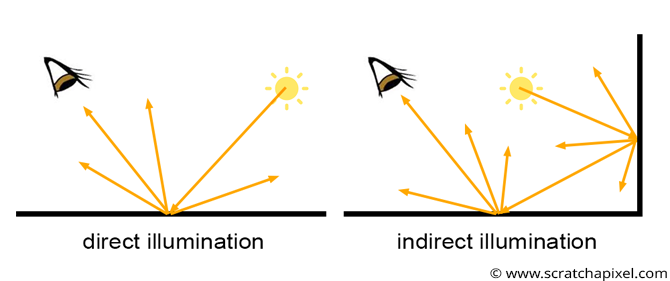
\includegraphics[scale=0.45]{media/shad2-globalillum3.png}
	\caption{Ejemplo de \textit{Iluminación directa e Iluminación indirecta}. Fuente: ScratchPixel}
	\label{globalil}
\end{figure}

\ref{item:dl} La iluminación directa es aquella que incide en un punto desde el foco de luz. \\
\ref{item:il} La iluminación indirecta es aquella que incide en un punto proveniente de la luz que rebota en otros puntos de la escena.

Recuperando lo expuesto en la introducción, el primer método capaz de renderizar imágenes realistas fue el \textit{Ray Tracing}, basado en la técnica de \textit{Ray Casting} de trazar rayos desde el observador a todos los pixeles de la imagen. La gran novedad respecto al algoritmo presentado por \citep{Appel1968} es la incorporación de la recursividad. En el \textit{Ray Tracing} se emite un rayo desde una cámara virtual hacia la escena para trazar el camino hasta los diferentes focos de luz de la escena. Cuando un rayo impacta contra un superficie puede generar tres tipos de rayos nuevos: \begin{enumerate*}[label=\roman*)] \item rayo de reflexión \label{ray:reflected}, \item rayo de refracción y \item rayo de sombra \end{enumerate*}. A partir de este punto, un nuevo rayo se proyecta hasta dar con las diferentes fuentes de luz de la escena. Al trazar los rayos nuevos somos capaces de conseguir efectos como reflejos, sombras, etc. debido a que para calcular el color estamos teniendo en cuenta como los demás objetos de la escena se afectan entre si. En caso de impactar con una superficie transparente, el rayo se proyecta a través de ésta para simular el efecto de refracción. Una gran desventaja de este método es la dependencia que éste tiene respecto a los polígonos de la escena; a más compleja es, más ineficiente será. 

A pesar de ofrecernos un alto grado de realismo al ser capaz de tratar con precisión efectos ópticos como la refracción, reflexión, los resultados obtenidos en una imagen renderizada mediante \textit{Ray Tracing} no son necesariamente foto-realistas. Se necesita hacer un postprocesado para simular efectos como sombras suaves (\textit{soft shwadows}, cáustica (\textit{caustics}), etc. Para conseguir renderizar imágenes foto-realistas, y por tanto efectos como cáusticas, debemos aproximar la RE, un buen ejemplo de ello es el método de \textit{Path Tracing} presentado por \citep{Kajiya1986}.

El algoritmo de \textit{Path Tracing} surge como mejora del \textit{Ray Tracing} con el objetivo de dar una solución a la RE mediante la integración de Monte Carlo. Es gracias a ésto que el algoritmo es capaz, de forma natural, representar efectos como \textit{Motion Blur}, \textit{Ambient Oclussion} e iluminación indirecta sin necesidad de posprocesado. A diferencia del \textit{Ray Tracing}, en el \textit{Path Tracing} cuando se emite un rayo desde la cámara virtual en vez de trazar el camino hasta los focos de luz de la escena, lo que hacemos es dejar que siga rebotando hasta golpear una fuente de luz o agotar un límite de profundidad en el número de rebotes que el rayo puede realizar. Pero la mayor diferencia respecto al método de Whitted es que en vez de tener en cuenta solamente el camino del rayo primigenio que emitimos, lanzamos decenas, cientos e incluso miles de rayos por pixel. Una característica importante del método de Kajiya es el muestreo aleatorio, esto significa que cuando un rayo impacta con una superficie éste genera uno nuevo en una dirección totalmente aleatoria. Una vez el rayo alcanza el límite de rebotes o es absorbido (por una fuente de luz) se calcula un valor en función de los objetos con los que rebotó y se añaden al promedio del pixel origen. Esta aleatoriedad provoca un resultado ruidoso que disminuye a medida que utilizamos más y más muestras por cada pixel.

\begin{figure}[!ht]
	\centering
	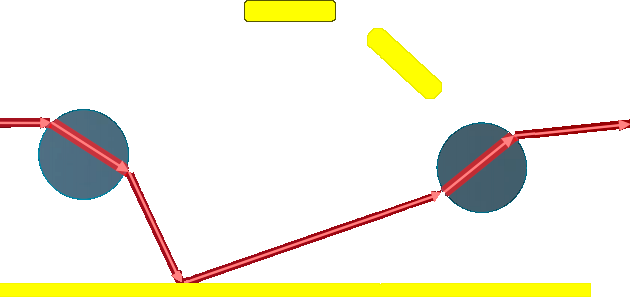
\includegraphics[scale=0.45]{media/lightPathRT.png}
	\caption{Trazado de rayo en \textit{Ray Tracing}.}
	\label{RT_traced}
\end{figure}

\begin{figure}[!ht]
	\centering
	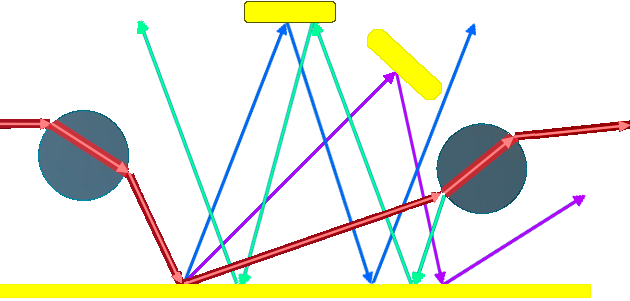
\includegraphics[scale=0.45]{media/lightPathPT.png}
	\caption{Trazado de rayo en \textit{Path Tracing}.}
	\label{PT_traced}
\end{figure}

En la Figura \ref{RT_traced} podemos observar aquello que comentamos en el párrafo anterior. En el \textit{Ray Tracing} el cálculo del color en un pixel solamente depende del trazado del rayo primario y como éste rebota por la escena hasta toparse con una fuente de luz. En cambio en la Figura \ref{PT_traced} se observa que a cada rebote, se generan múltiples rayos (en la imagen se ilustran un pequeña muestra). Esto ocurre porque cuando un rayo impacta contra una superficie difusa los fotones se dispersan en todas direcciones. Estos nuevos rayos nos permiten calcular la iluminación global para ofrecernos así un mayor realismo. 

El \textit{Path Tracing} es indiferente al número de polígonos presentes en la escena, la complejidad de la escena no afecta proporcionalmente al rendimiento del algoritmo. Como hemos mencionado anteriormente, en el primer método se traza un rayo por cada polígono de la escena, en cambio en el método de Kajiya el rayo se traza por pixel. Debido a que cada uno es independiente de los demás, tenemos un algoritmo con una alta capacidad de paralelismo. En consecuencia, podemos explotar la capacidad de concurrencia que nos proporcionan las CPUs y GPUs; y poder así calcular más de un pixel de la imagen al mismo tiempo.

\begin{figure}[H]
	\centering
	\begin{subfigure}{.3\textwidth}
		\centering
		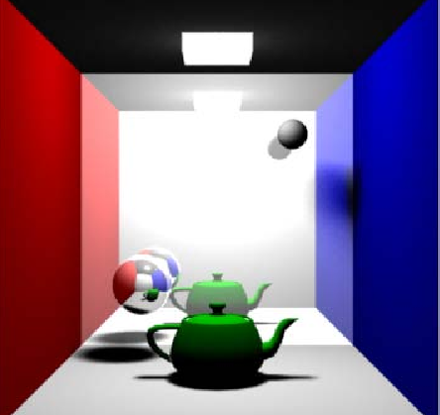
\includegraphics[width=.8\textwidth]{media/RayTracing.png}
		\caption{\textit{Ray Tracing}.}
		\label{RT}
	\end{subfigure}
	\begin{subfigure}{.3\textwidth}
		\centering
		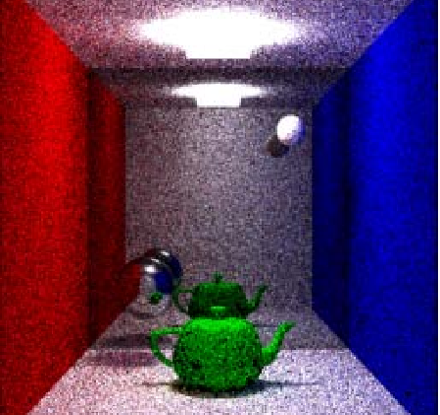
\includegraphics[width=.8\textwidth]{media/PathTracing.png}
		\caption{\textit{Path Tracing} con ruido.}
		\label{PTN}
	\end{subfigure}
	\begin{subfigure}{.3\textwidth}
		\centering
		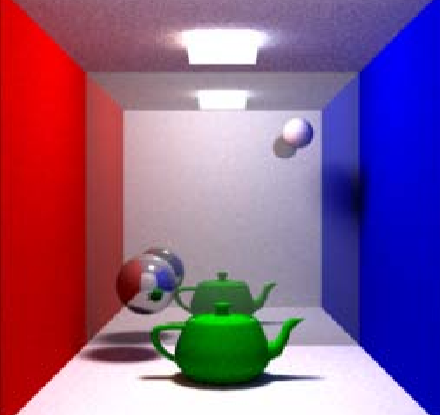
\includegraphics[width=.8\textwidth]{media/PathTracingMD.png}	
		\caption{\textit{Path Tracing} sin ruido.}
		\label{PT}
	\end{subfigure}
	\caption{Comparación \textit{Ray Tracing vs. Path Tracing}. Fuente: \citep{Cassagnabere2004}}
\end{figure}

Podemos apreciar como el \textit{Path Tracing}, Figura \ref{RT}, produce una sombras más suaves respecto al \textit{Ray Tracing}, Figura \ref{PT}. También se puede observar el efecto de ruido que provoca \textit{Path Tracing}, Figura \ref{PTN}, si pocas muestras por pixeles son utilizadas.

En el presente proyecto trataremos de crear un aplicación que implemente el método de \textit{Path Tracing} para generar imágenes de carácter realista. Dicha aplicación calculará cada pixel de la imagen final de forma secuencia, es decir, uno tras otro y nos servirá de base para crear una solución paralela haciendo uso de la GPU y otra haciendo uso de la CPU. El porque de realizar estas tres aplicaciones es para ser capaces de realizar un análisis del rendimiento que nuestro algoritmo obtiene explorando en profundidad la capacidad de concurrencia que nos ofrecen a día de hoy las CPUs y GPUs; y ver así que arquitectura nos ofrece mayor rendimiento.

Como base, partiremos de la implementación propuesta por Peter Shirley en su ''saga'' de libros sobre \textit{Ray Tracing} \citep{ShirleyRTA, ShirleyRTB, ShirleyRTC} para implementar nuestro \textit{Path Tracing}. La idea principal es desarrollar tres aplicaciones (una secuencia, una paralela en CPU y otra paralela en GPU) partiendo de la base que nos presenta Shirley, para poder hacer un análisis que como es el rendimiento de un \textit{Path Traing} explotando la capacidad de concurrencia de una CPU contra la de una GPU.

No solo nos centraremos en el apartado de renderizado, aunque se trata de la trama central de este proyecto, sino que estudiaremos también que técnicas de aceleración son comúnmente utilizadas para tratar de mejorar al máximo nuestro algoritmo. Es por ello que veremos también cual es la mejor manera de representar de forma interna la escena que queremos renderizar siguiendo la idea que nos presenta \citep{Karras2012} en su artículo.

La forma en que representemos nuestra escena tendrá un gran impacto a la hora de calcular el color de la imagen final. Como hemos comentado, la base del método es trazar rayos por la escena para calcular el color de cada pixel. Si nuestra representación de la escena consiste en almacenar todos los objetos en una estructura de datos de tipo lista o vector ordenados por orden de creación, a la hora de calcular un punto de la imagen en el peor caso estaremos recorriendo todo el conjunto de polígonos de la escena para determinar el color final. Tratar de renderizar una escena que, muy posiblemente, esté compuesta de millones de polígonos puede traducirse en horas y horas de procesado. Es por eso que haremos uso de una estructura de datos aceleradora que nos permita representar la escena de una forma más inteligente, para que a la hora de determinar si un rayo impacta o no un polígono se determine de la forma más rápida posible

\section{Justificación}

Como bien hemos indicado en la sección anterior, partiremos de los libros presentados por Peter Shirley y el artículo sobre \textit{Bounding Volume Hierarchy} de Tero Karras para construir nuestras aplicaciones. En este trabajo lo que pretendemos es estudiar como podemos explotar al máximo las diferentes arquitecturas que tenemos en nuestra computadora (CPU y GPU) y ver en cual de ellas un método de renderizado de imágenes realistas se comporta de manera más eficiente. No podremos comparar nuestra solución aportada frente otras aplicaciones existentes que implementan también el método de \textit{Path Tracing} en GPU o CPU. En el ámbito de comparación de eficiencia en ciertas partes de la aplicación, como por ejemplo comprar el rendimiento del cálculo de la imagen final dada la representación de una escena, es difícil de comparar con aplicaciones que podrían ser similares debido que éstas están desarrolladas por expertos en la materia con una amplía experiencia y una serie de conocimientos que el autor del presente proyecto no tiene. Este conocimiento y experiencia les permite aplicar una serie de técnicas de optimización que pueden aumentar el rendimiento de forma notable. En el ámbito del realismo que podemos conseguir respecto el que consiguen otras aplicaciones también es complicado de comparar. La mayoría de aplicaciones que implementan un \textit{Path Tracing} no sólo implementan dicho método, sino que también implementan mucho más efectos, como por ejemplo \textit{subsurface scatering}. En el presente proyecto es imposible lograr una aplicación de características similares, primero por la falta de conocimiento o experiencia en el campo de renderización realista y segundo por el tiempo. Normalmente, un proyecto de estas dimensiones involucran a varios expertos en la materia y se disponen de más tiempo de realización. Un ejemplo de aplicación profesional es RenderMan de Pixar Animation Studios \citep{Christensen2018}.

Por esto mismo, en el presente proyecto realizaremos tres versiones del mismo algoritmo: \begin{enumerate*}[label=\roman*)] \item versión secuencial, \item versión paralela en CPU y \item versión paralela en GPU \end{enumerate*}. De esta forma podremos hacer una comparativa de que arquitectura nos brinda una mayor ventaja para nuestra implementación.

En la actualidad son muchas las librerías orientadas a la programación en GPU. Tenemos librerías como \texttt{OpenCL} y \texttt{OpenACC}, que nos permiten una mayor portabilidad entre tarjetas gráficas de distintos fabricantes como por ejemplo \texttt{AMD} y \texttt{NVIDIA}. Pero para este proyecto hemos decidido escoger el entorno de \texttt{CUDA} desarrollado por \texttt{NVIDIA} específicamente para sus tarjetas gráficas y aceleradores. Decidimos usar esta API debido a que se trata de software propietario, mejor optimizado para las tarjetas de dicha empresa como bien nos indican \citep{Karimi2010} y \citep{Fang2011} respectivamente en sus artículos científicos, las cuales utilizaremos en este proyecto.

Es posible que, citadas tarjetas/aceleradores \texttt{NVIDIA} y, teniendo presente que el proyecto está enfocado al tema de renderizado de gráficos realistas, al lector del presente Trabajo de Fin de Grado le venga a la mente la nueva gama de tarjetas RTX diseñadas por \texttt{NVIDIA}. En un inicio se planteó guiar el proyecto hacia el uso de tarjetas con tecnología RTX debido a que éstas han sido diseñadas específicamente para el uso de \textit{Ray Tracing} en tiempo real. Pero esta idea fue descartada en seguida debido al elevado precio de éstas. El rango de precios de las tarjetas de esta gama oscila entre los 350€ en los modelos más económicos, hasta los varios miles de euros en modelos destinados a entornos profesionales. Finalmente, aunque el autor de dicho trabajo adquirió una tarjeta gráfica NVIDIA RTX 280 Super con 8Gb de memoria, se decidió no guiar el proyecto a utilizarla de forma exclusiva, estudiando y poniendo en práctica las nuevas mejoras que ésta ofrece (RT Cores, Tensor Cores, Mesh Shaders, etc.), frente a otras tarjetas de gamas inferiores que no incluyen, debido al corto plazo de tiempo para el desarrollo. Es por eso que esta tarjeta gráfica será usada para testar nuestra aplicación, pero no en un sentido exclusivo. Enfocar el trabajo a explorar en profundidad las nuevas características introducidas no fue posible, hubiera significado reestructurar todo el proyecto desde cero. Esto hubiera supuesto una gran perdida del tiempo invertido en adquirir los conocimientos necesarios para realizar el presente proyecto, es por eso que no se decidió enfocar el trabajo en el gran potencial que nos brinda la tecnología RTX. Eso no quiere decir que no podamos utilizarla. Al ser una tarjeta gráfica de gama alta, el número de cores que tiene respecto a la GTX1050 (gama media) nos permitirá analizar cuan mejor es y si merece o no la pena, en relación coste-potencia, su uso en aplicaciones de este tipo.

Como hemos comentado al inicio de esta sección, \texttt{CUDA} es un API que está muy bien optimizada para hardware de \texttt{NVIDIA}. Esto nos da un punto a favor debido a que la aplicación que vamos a desarrollar será probada en diferentes entornos que utilizan la tecnología de NVIDIA:

\begin{enumerate}
	\item Computador portátil - Lenovo Legion Y520 con Nvidia GTX1050 Mobile - 4GB.
	\item Computador personal - Nvidia RTX 2080 Super - 8Gb.
	\item Cluster docencia BOADA - 4 GPUs Nvidia Tesla K40c.
\end{enumerate}

Al usar tarjetas en entornos diferentes podremos analizar como nuestra aplicación responde en cada uno de ellos y estudiar así cómo es el rendimiento cuando utilizamos varias tarjetas pensadas para un entorno de investigación/profesional, en contraposición con otras dos pensadas para un uso más cotidiano. También podremos ver como es el rendimiento en una tarjeta gráfica de gama media (Nvidia GTX1050 Mobile) y una de gama alta (Nvidia RTX 2080 Super); y hacer así una comparativa entre ellas.

\section{Planificación}

Hemos seguido la planificación especificada en el informe de la fase inicial, permitiéndonos un poco de flexibilidad en cuanto al inicio de las tareas de forma que pudiéramos empezar tan pronto posible el desarrollo del proyecto. Esto nos ha permitido poder llevar a cabo diferentes tareas independientes en paralelo e ir cumpliendo los objetivos propuestos en cada una de las reuniones de seguimiento realizadas hasta el momento de la presente entrega.

En la fase final es dónde reuniéremos los resultados de todos los experimentos realizados en cada una de las fases y sacar las conclusiones adecuadas para cada uno de ellos y de esta forma redactar la memoria final del proyecto.

\subsection{Diagrama de Gantt}

\uselandscape

\begin{figure}[H]
	\centering
	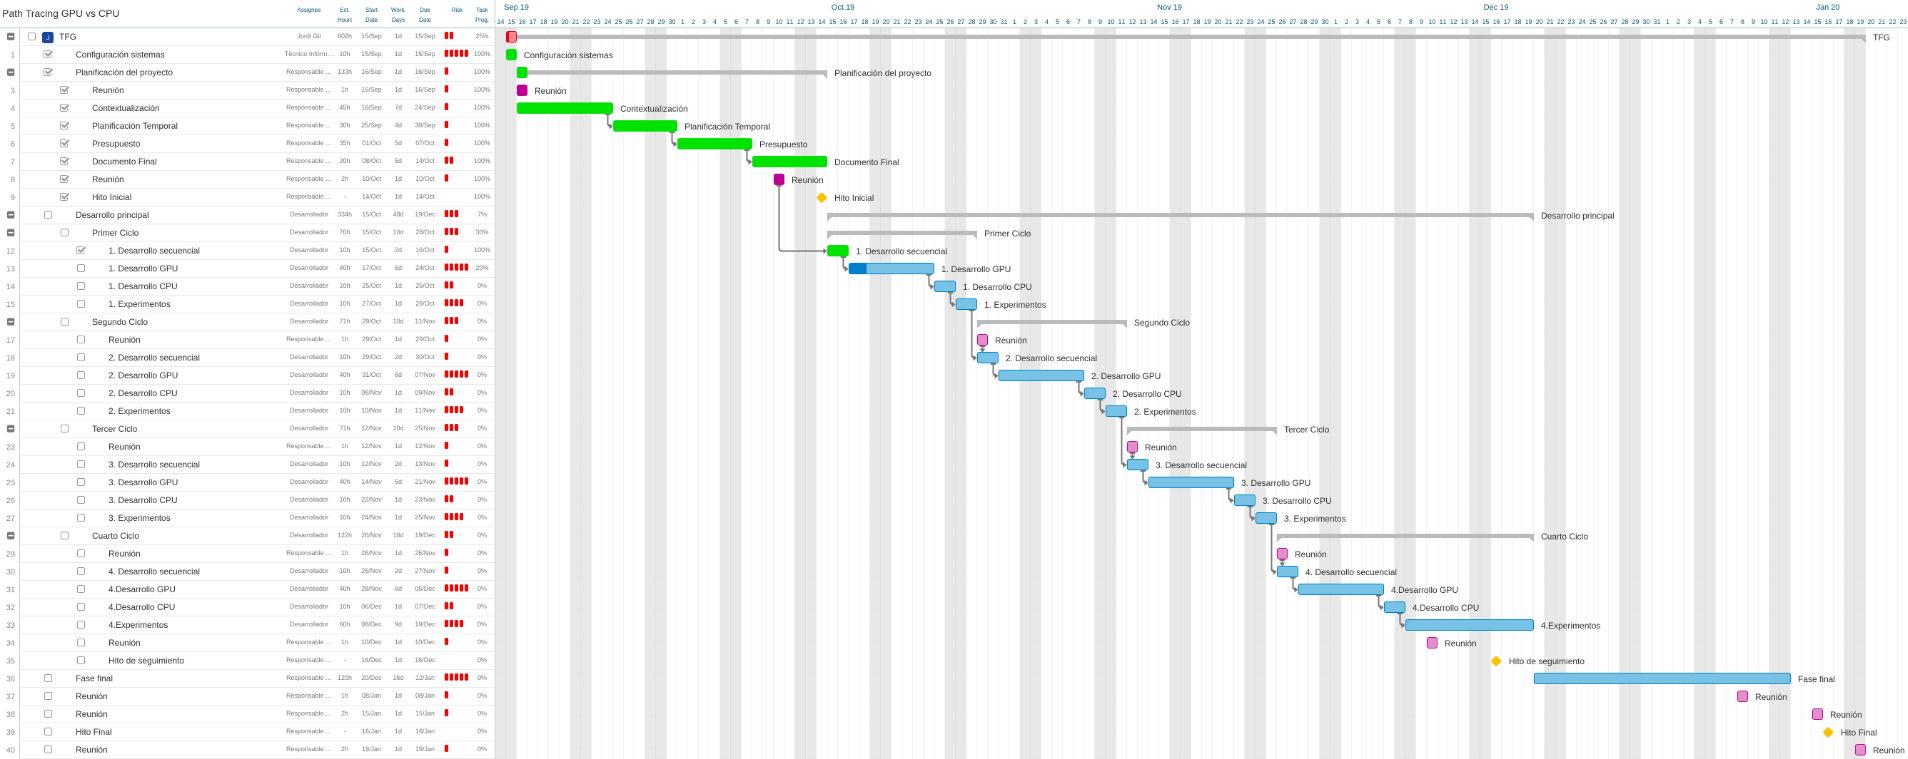
\includegraphics[scale=1.45]{media/final_gantt.png}
	\captionof{figure}{Diagrama de Gantt completo.}
	\label{gantt}
\end{figure}

\begin{figure}[H]
	\centering
  	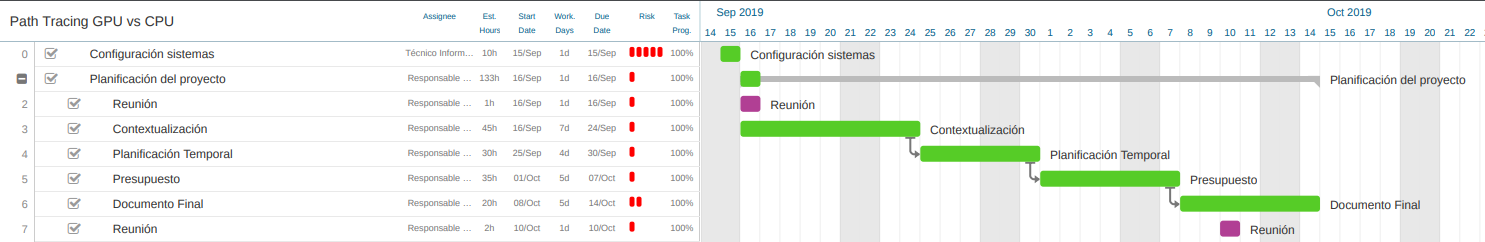
\includegraphics[scale=1.5]{media/final_gantt_1.png}
  	\captionof{figure}{Etapa de gestión.}
  	\label{gantt_1}
\end{figure}

\begin{figure}[H]
	\centering
  	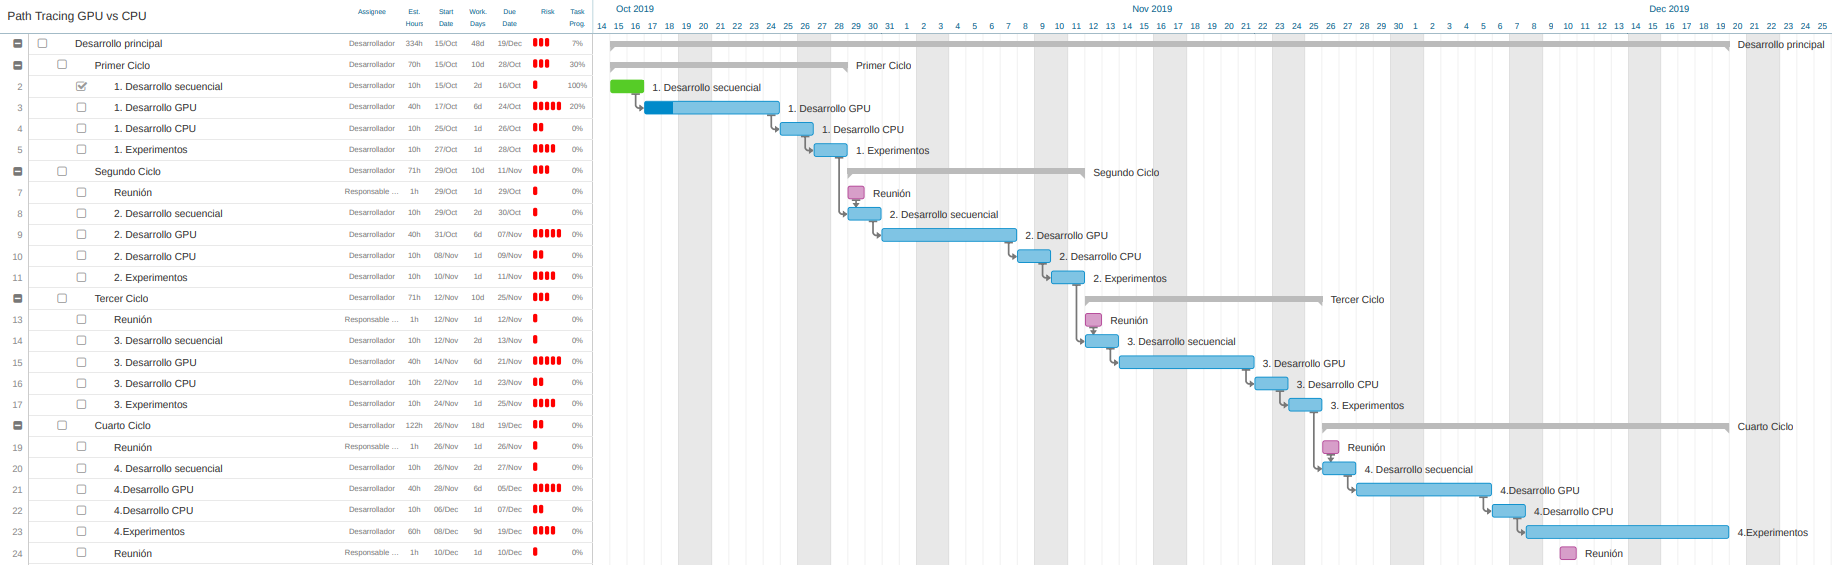
\includegraphics[scale=1.25]{media/final_gantt_2.png}
  	\captionof{figure}{Etapa de desarrollo.}
  	\label{gantt_2}
\end{figure}

\useportrait

\section{Metodología}

La metodología usada es la misma que la escogido al inicio del proyecto. Esta nos ha permitido ir desarrollando el proyecto por fases para así poder tener una visión general del estado proyecto.

\section{Análisis de alternativas}

Durante la planificación del proyecto se definieron de forma clara y concisa cuales son los objetivos principales del proyecto. Esto nos ha permitido saber en todo preciso momento que objetivos se han cumplido y cuales no.

Además, en el caso de no poder disponer de diferentes formas (\textit{shapes}) con las cuales poder definir los objetos 3D de nuestra escena tales como: esferas, triángulos, discos. Utilizaremos solamente triángulos debido a la versatilidad que estos nos proporcionan para renderizar mayas de triángulos (y que pueden definir las otras formas).

\section{Integración de conocimientos}

Principalmente, los conocimientos integrados en el presente proyecto corresponden a los adquiridos en la especialidad de computación, así como alguna asignatura obligatorio del grado y otras optativas. Se han requerido conocimientos en renderización realistas y aplicación de transformaciones geométricas sobre objetos 3D vistos en la asignatura de gráficos. O, por otro lado, aspectos como la creación de programas paralelos en una CPU haciendo uso de \texttt{OpenMP}, vistos en la asignatura de paralelismo, o en una GPU de \textit{NVidia} haciendo uso del entorno de \texttt{CUDA}, vistos en la asignatura de Tarjetas Gráficas y Aceleradores.

El conocimiento en programación ha sido necesario para poder llevar a cabo el desarrollo de las diferentes versiones de nuestro proyecto. En concreto, conocimientos en lenguajes como \texttt{C} y \texttt{C} han sido necesarios para el buen desarrollo del presente proyecto.

\section{Identificación de leyes y regulaciones}

Como bien comentamos en la primera entrega, el objetivo de este proyecto no es realizar ningún tipo de producto, sino más bien permitir al autor de este entrar en al gran mundo de la renderización por computador, en concreto la renderización realista. Es por todo esto que no hay ningún tipo de leyes o regulaciones que puedan ser aplicadas. Además, el material i/o herramientas utilizados a lo largo de todo el proyecto son de dominio público o de creación propia.


\newpage

\printbibliography

\listoffigures

\listoftables

\end{document}
